\documentclass[letterpaper,12pt]{article}

\usepackage{geometry, pslatex, fancyhdr, graphicx}
\usepackage{amsmath,amsthm,amssymb,scrextend}
\usepackage{multicol}
\usepackage{tabularx}
\usepackage[makeroom]{cancel}
\usepackage{color}
\geometry{ margin = 1.0in }

%%% TODO modify these variables as per your homework %%%
\def\homeworknum{1}
\def\myname{Harshit Jain}
\def\myuserid{hmj5262}
%%%%

\pagestyle{fancy}
\lhead{{\bf CMPSC 464 Spring 2024}}
\chead{{\bf Assignment~\homeworknum}}
\rhead{{\bf \today}}
\let\newproof\proof
\renewenvironment{proof}{\begin{addmargin}[1em]{0em}\begin{newproof}}{\end{newproof}\end{addmargin}\qed}

\newcounter{problemid}
\stepcounter{problemid}
\def\newproblem{\clearpage\newpage{\bf Problem~\arabic{problemid}\stepcounter{problemid}}\hfill\par}

\setlength\parindent{0em} 
\setlength\parskip{8pt}
\setlength{\fboxsep}{6pt}


\begin{document}

\framebox[\textwidth]{
	\parbox{0.96\textwidth}{
		\parbox{0.12\textwidth}{\bf Name:}\parbox{0.6\textwidth}{\myname}\\
		\parbox{0.12\textwidth}{\bf User ID:}\parbox{0.6\textwidth}{\myuserid}
	}
}

I collaborated with Yug Jarodiya and Beniamin Margaryan.
%% your solutions %%%


% PROBLEM 1
\newproblem 
\begin{enumerate}
    \item 
    Let's suppose $\sqrt{13}$ is a rational number. Then we can write it $\sqrt{13} = \frac{a}{b}$ where $a, b$ are whole numbers, $b$ not zero.

    We additionally assume that this $\frac{a}{b}$ is simplified to lowest terms, since that can obviously be done with any fraction. Notice that in order for $\frac{a}{b}$ to be in simplest terms, both of $a$ and $b$ cannot be even. One or both must be odd. Otherwise, we could simplify $\frac{a}{b}$ further.

    From the equality $\sqrt{13} = \frac{a}{b}$ it follows that $13 = \frac{a^2}{b^2}$,  or  $a^2 = 13b^2$. Since $13$ is prime and $a^2$ is a multiple of $13$, then $a$ is multiple of $13$.

    If we substitute $a = 13k$ into the original equation $\sqrt{13} = \frac{a}{b}$, we get:

    $\Rightarrow (13k)^2 = 13b^2$

    $\Rightarrow b^2 = 13k^2$

    Since $13$ is prime and $b^2$ is a multiple of $13$ then $b$ is multiple of $13$.

    We now have a contradiction since $a$ and $b$ must have no common factors (except $1$) but we have proved that if $\frac{a}{b}$ exits then $a$ and $b$ must have common factor $13$.
    
    So $\frac{a}{b}$ can not exist and the square root of $13$ is irrational.
    
    \item Yes, we can prove that square root of any prime number is irrational.

    Let's suppose $\sqrt{p}$ is a rational number, where $p$ is any prime number. Let $\sqrt{p} = \frac{m}{n}$ where $m,n \in N$. and $m$ and $n$ have no factors in common.

    Now $p = \frac{m^2}{n^2}$,  or  $m^2 = pn^2$.
    
    Since $p$ is prime and $m^2$ is a multiple of $p$ then $m$ is multiple of $p$.
    
    If we substitute $m = pk$ into the original equation $\sqrt{p} = \frac{m}{n}$, we get:
    
    $\Rightarrow (pk)^2 = pn^2$

    $\Rightarrow n^2 = pk^2$
    
    Since $p$ is prime and $n^2$ is a multiple of $p$ then $n$ is multiple of $p$.
    
    We now have a contradiction since $m$ and $n$ must have no common factors (except $1$) but we have proved that if $\frac{m}{n}$ exits then $m$ and $n$ must have common factor $p$.
    
    So $\frac{m}{n}$ can not exist and the square root of any prime is irrational.

\end{enumerate}

% PROBLEM 2
\newproblem
$Q = \{ q_0, q_1, q_2, q_3 \}$

$q_0:$ State after reading a digit that leaves a remainder of $0$ when divided by $4$ \\
$q_1:$ Initial State, State after reading a digit that leaves a remainder of $1$ when divided by $4$ \\
$q_2:$ State after reading a digit that leaves a remainder of $2$ when divided by $4$ \\
$q_3:$ State after reading a digit that leaves a remainder of $3$ when divided by $4$

$\Sigma = \{ 0, 1, 2, 3 \}$

$q_0 = \{ q_1 \}$ (Start State)

$F = \{ q_0 \}$ (Accept State)

$\delta =$ 
\begin{tabular}{c|cccc}
    & 0 & 1 & 2 & 3 \\
    \hline
    $q_0$ & $q_0$ & $q_0$ & $q_0$ & $q_0$ \\
    $q_1$ & $q_0$ & $q_1$ & $q_2$ & $q_3$ \\
    $q_2$ & $q_0$ & $q_2$ & $q_0$ & $q_2$ \\
    $q_3$ & $q_0$ & $q_3$ & $q_2$ & $q_1$ \\
\end{tabular}

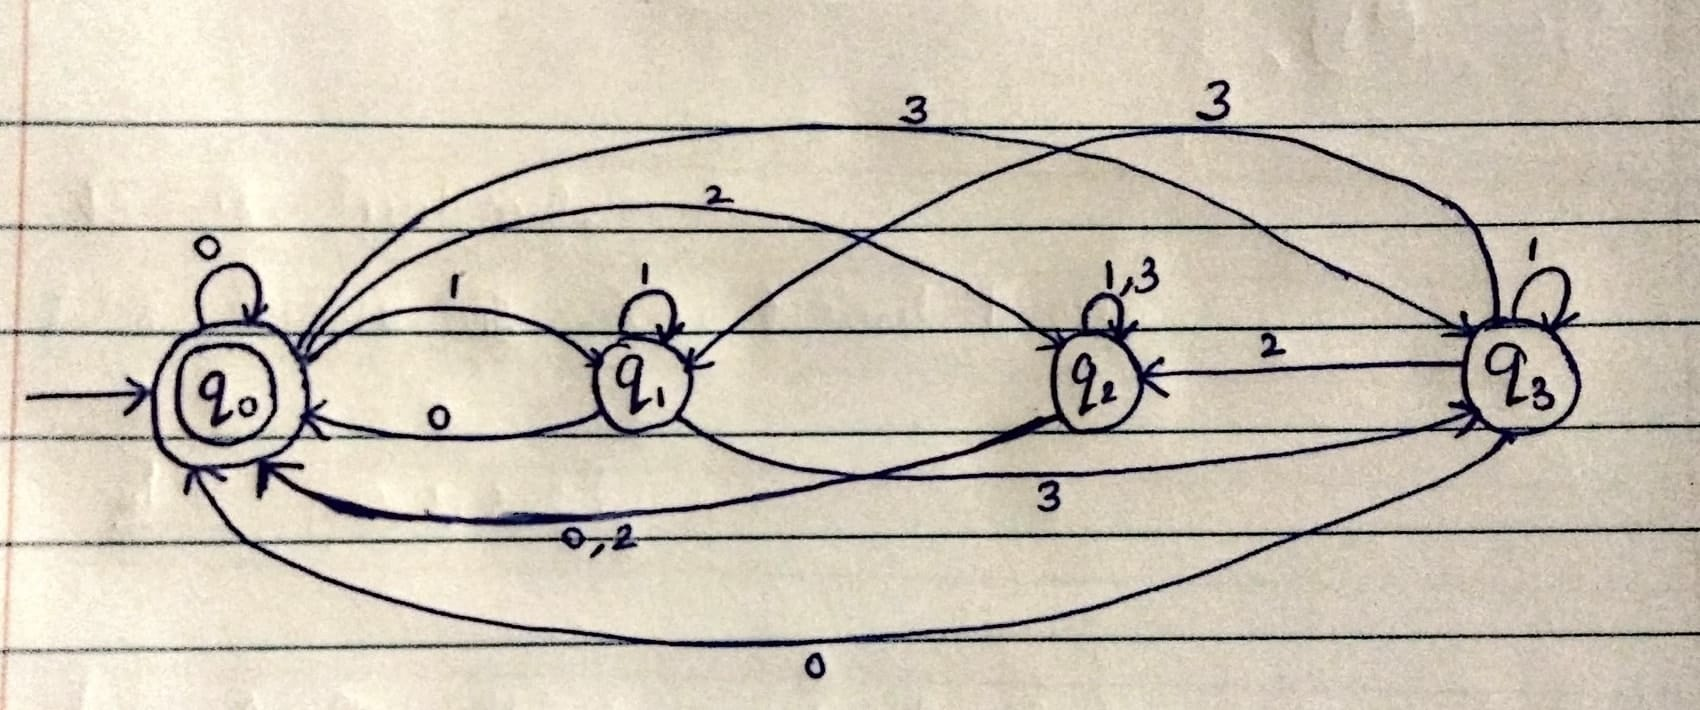
\includegraphics[scale = 0.20]{2}

% PROBLEM 3
\newproblem
\begin{enumerate}
    \item 
    Assume there exists a DFA over the alphabet $\{ 0, 1 \}$ that recognizes the language $L = \{ 1 \}$ with less than three states.

    A DFA has states, transitions, an initial state, and accepting states. Let's analyze the possibilities:

    \begin{itemize}
        \item We must have at least one start state. Let the start state be $q_0$.
        \item For the string $1$, there must be an accepting state. Let this state be $q_1$.
        \item Let's introduce a dead state to $q_{dead}$ handle strings other than $1$. This state will be a non-accepting state, and we can transition to it from $q_0$ to $q_1$ on input $0$ or $1$.
    \end{itemize}

    Now, this DFA has three states: $q_0$, $q_1$, and $q_{dead}$. It ensures that only the string "1" is accepted, and all other strings lead to the dead state.

    Therefore, we have shown that it is impossible to create a DFA with less than three states that recognizes the language $L = \{ 1 \}$, and we need at least three states, including a dead state, to handle strings other than 1.
    
    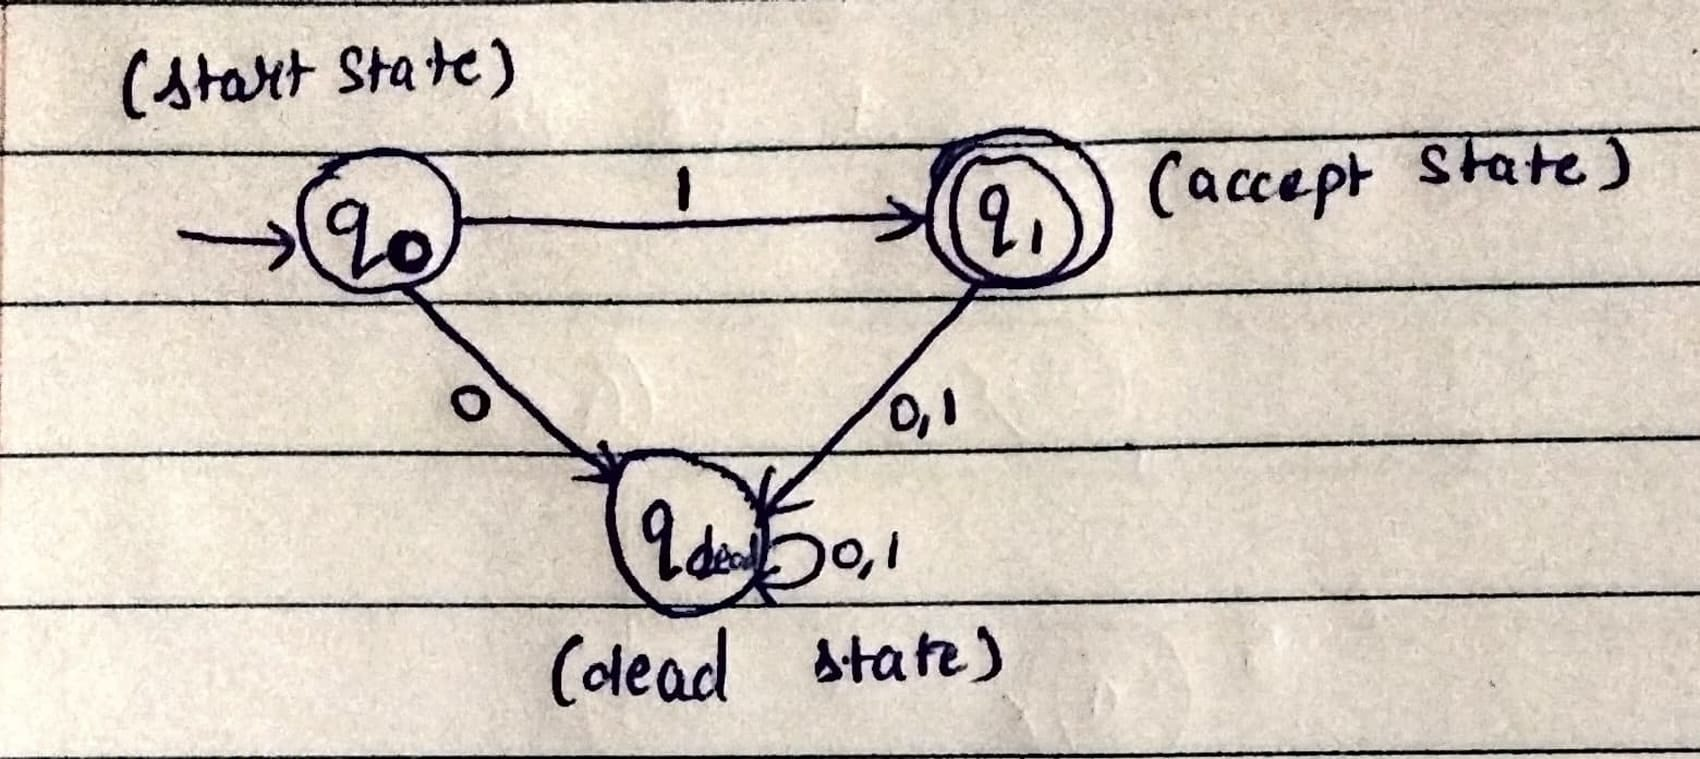
\includegraphics[scale = 0.20]{3a}

    \item 
    Yes, the DFA over the alphabet $\{ 1 \}$ that recognizes the language $L = \{ 1 \}$ needs to have at least three states.

    \underline{States:}
    \begin{itemize}
        \item $q_0$ (Start state)
        \item $q_1$ (Accept state for the valid string 1)
        \item $q_{dead}$ (Dead state for any other invalid string)
    \end{itemize}

    \underline{Transitions:}
    \begin{itemize}
        \item From $q_0$, on input $1$, transition to $q_1$
        \item From $q_1$, on input $1$, transition to $q_{dead}$
    \end{itemize}

    This DFA ensures that only the string $1$ is accepted (transitioning from $q_0$ to $q_1$), and any additional $1$s are rejected by transitioning to the dead state $q_{dead}$. Thus, a minimum of three states is required to handle both acceptance and rejection of strings in the language $L = \{ 1 \}$ over the alphabet $\{ 1 \}$.

    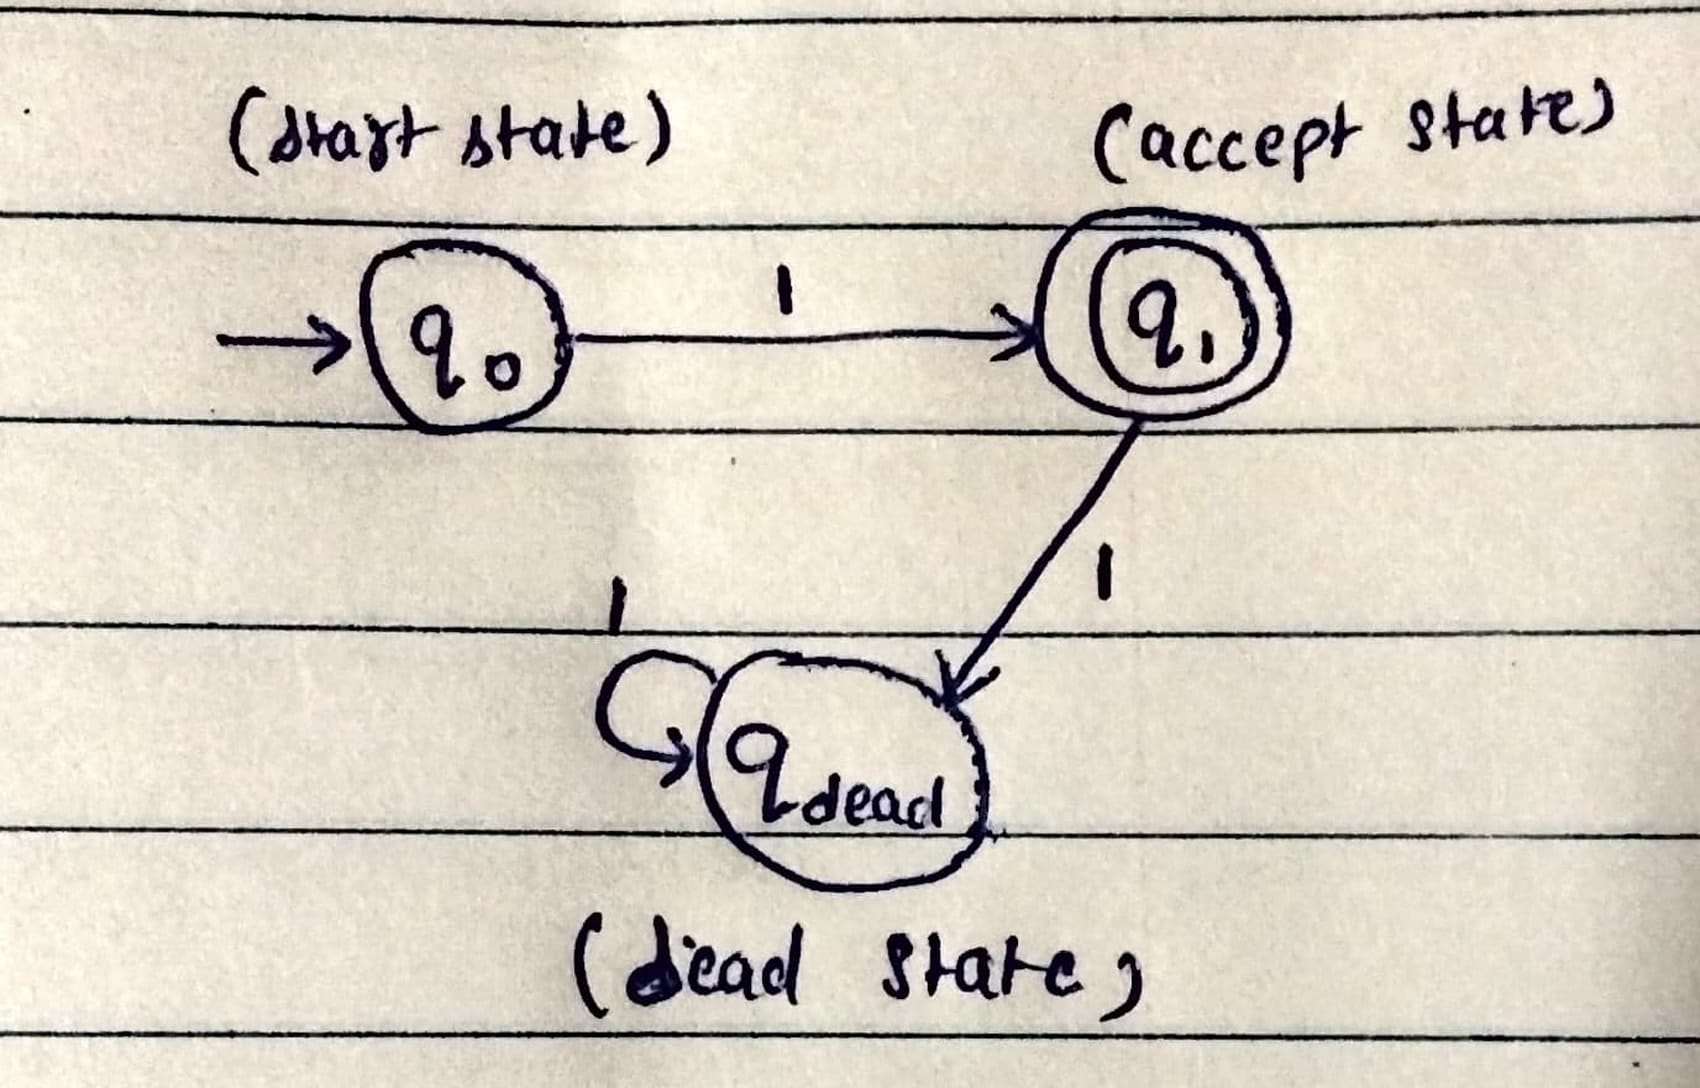
\includegraphics[scale = 0.20]{3b}
\end{enumerate}

% PROBLEM 4
\newproblem
From the given NFA, we will make the transition table, $\delta_{NFA} = $
\begin{tabular}{c|cccc}
    & a & b \\
    \hline
    $1$ & $\{1,2\}$ & $2$ \\
    $2$ & $\phi$ & $1$ \\
\end{tabular}

From here, we can make an equivalent DFA transition table as follows, $\delta_{DFA} = $
\begin{tabular}{c|cccc}
    & a & b \\
    \hline
    $1$ & $12$ & $2$ \\
    $12$ & $12$ & $12$ \\
    $2$ & $D$ & $1$ \\
    $D$ & $D$ & $D$ \\
\end{tabular}

\underline{States:}
    \begin{itemize}
        \item $1$ (Start state and Accept State)
        \item $12$ (Accept state)
        \item $D$ (Dead state for any other invalid string)
    \end{itemize}

So, the converted DFA is as follows:

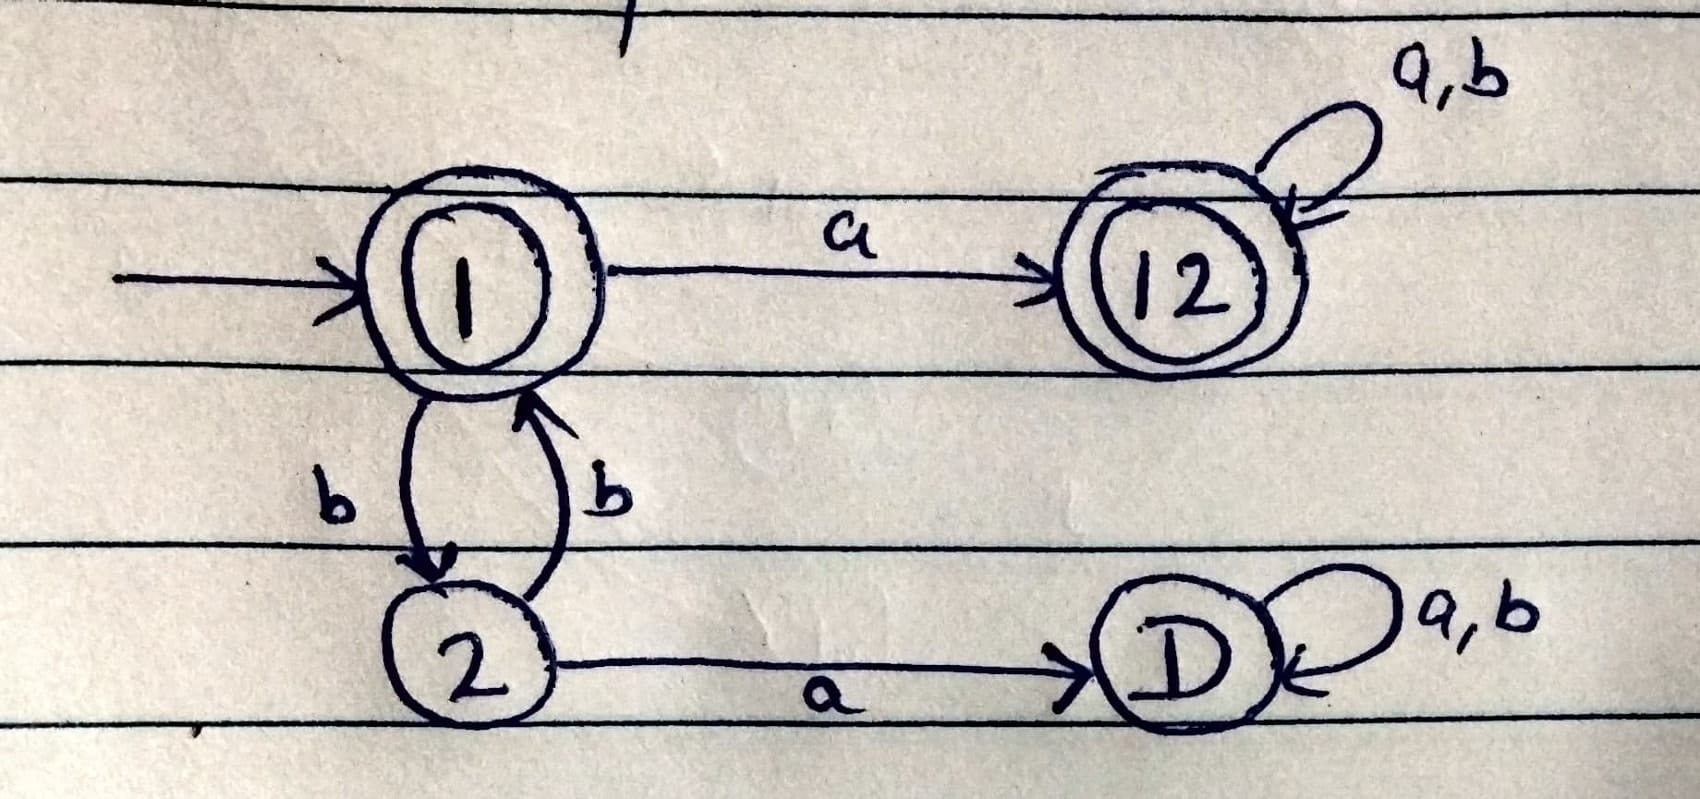
\includegraphics[scale = 0.20]{4}

% PROBLEM 5
\newproblem
\begin{enumerate}
    \item I am going for $30\%$
    \item 
    (adapted from Textbook- Page 55)

    PROOF. Let \(N = (Q, \Sigma, \delta, q_0, F)\) be the NFA recognizing some language \(A\). We construct a DFA \(M = (Q', \Sigma, \delta', q_0', F')\) recognizing \(A\). Suppose \(N\) has no \(\varepsilon\) arrows.

    \begin{itemize}
        \item \(Q' = P(Q)\). Every state of \(M\) is a set of states of \(N\). Recall that \(P(Q)\) is the set of subsets of \(Q\).
        
        \item For \(R \in Q'\) and \(a \in \Sigma\), let \(\delta'(R, a) = \{q \in Q | q \in \delta(r, a) \text{ for some } r \in R\}\). If \(R\) is a state of \(M\), it is also a set of states of \(N\). When \(M\) reads a symbol \(a\) in state \(R\), it shows where \(a\) takes each state in \(R\). Because each state may go to a set of states, we take the union of all these sets. Another way to write this expression is:
        \[\delta'(R, a) = \bigcup_{r \in R} \delta(r, a)\]

        \item \(q_0' = \{q_0\}\). \(M\) starts in the state corresponding to the collection containing just the start state of \(N\).

        \item \(F' = \{R \in Q' | R \text{ contains 4 accept states of } N\}\). The machine \(M\) accepts if 4 of the possible states that \(N\) could be in at this point is an accept state.
    \end{itemize}
    Now we need to suppose that there are \(\varepsilon\) arrows. For any state \(R\) of \(M\), we define \(E(R)\) to be the collection of states that can be reached from members of \(R\) by going only along \(\varepsilon\) arrows, including the members of \(R\) themselves. Formally, for \(R \subseteq Q\) let:
    \[E(R) = \{q | q \text{ can be reached from } R \text{ by traveling along 0 or more } \varepsilon \text{ arrows}\}.\]
    
    Then we modify the transition function of \(M\) to place additional fingers on all states that can be reached by going along \(\varepsilon\) arrows after every step. Replacing \(\delta(r, a)\) by \(E(\delta(r, a))\) achieves this effect. Thus:
    \[\delta'(R, a) = \{q \in Q | q \in E(\delta(r, a)) \text{ for some } r \in R\}.\]

    Additionally, we need to modify the start state of \(M\) to move the fingers initially to all possible states that can be reached from the start state of \(N\) along the \(\varepsilon\) arrows. Changing \(q_0'\) to be \(E(\{q_0\})\) achieves this effect. We have now completed the construction of the DFA \(M\) that simulates the NFA \(N\).

    The construction of \(M\) obviously works correctly. At every step in the computation of \(M\) on an input, it clearly enters a state that corresponds to the subset of states that \(N\) could be in at that point. Thus, our proof is complete.

    \item No, there is nothing inherently special about the number $4$ in the context of \(k\)-NFAs. The choice of $4$ in the question is arbitrary, and the same concept applies to \(k\)-NFAs for any \(k > 1\), including 3NFA or 5NFA.
    
    For any \(k\)-NFA, where \(k > 1\), the idea is that multiple branches or paths must reach an accept state for the input string to be accepted. If the question used 3NFA, the requirement would be that at least $3$ branches must reach an accept state. If it used 5NFA, the requirement would be that at least $5$ branches must reach an accept state.



\end{enumerate}
\end{document}